\chapter{Simulation}
\label{ch:simulation}

\section{Simulation Overview}
This simulation was developed by \cite{Sharma2013} using MATLAB and Simulink, for the purpose of tracking several ground targets. This was achieved by using a camera mounted in an aircraft and pointing it in an optimal fashion to improve the estimation of the states of all the objectives. A block was added to provide the means of pointing an antenna and a camera towards a UAV, estimating the states with a Delayed Extended Kalman Filter. In this study we are not concerned about the behavior of the plane, since we will point it as long as there is line-of-sight. The simulation has four main blocks: UAV Sensor Block, Target Selection Step, Antenna Pointer block, and 3-D Plot block. We will only focus on the block that we developed, the Antenna Pointer block.

\begin{figure}[h!]
  %\centering
  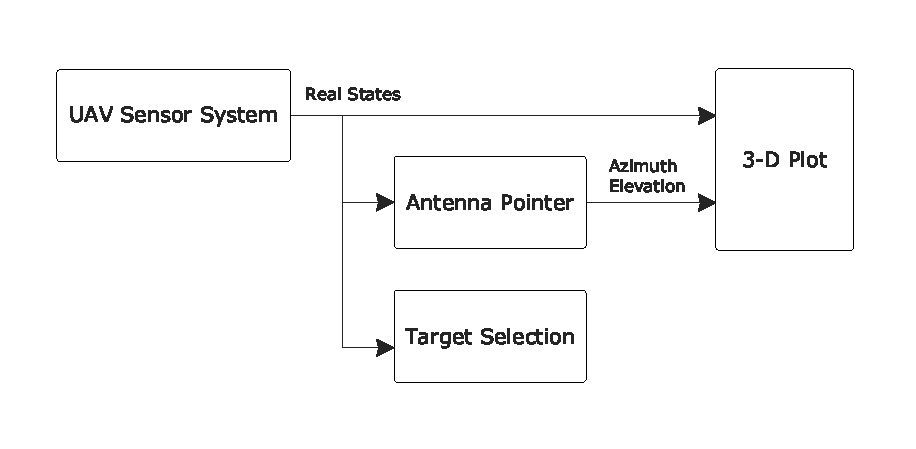
\includegraphics[scale=0.9]{./Simulink/system_overview.eps}
  \label{fig:system_overview}
  \caption[Antenna Pointer Block]{Antenna Pointer Block}
\end{figure}


\section{Antenna Pointer}
The antenna pointer block points precisely an antenna and a camera towards the aircraft. It consists of four blocks: GPS, camera, EKF/DEKF and a pointer block as shown below.
 
\begin{figure}[h!]
  %\centering
  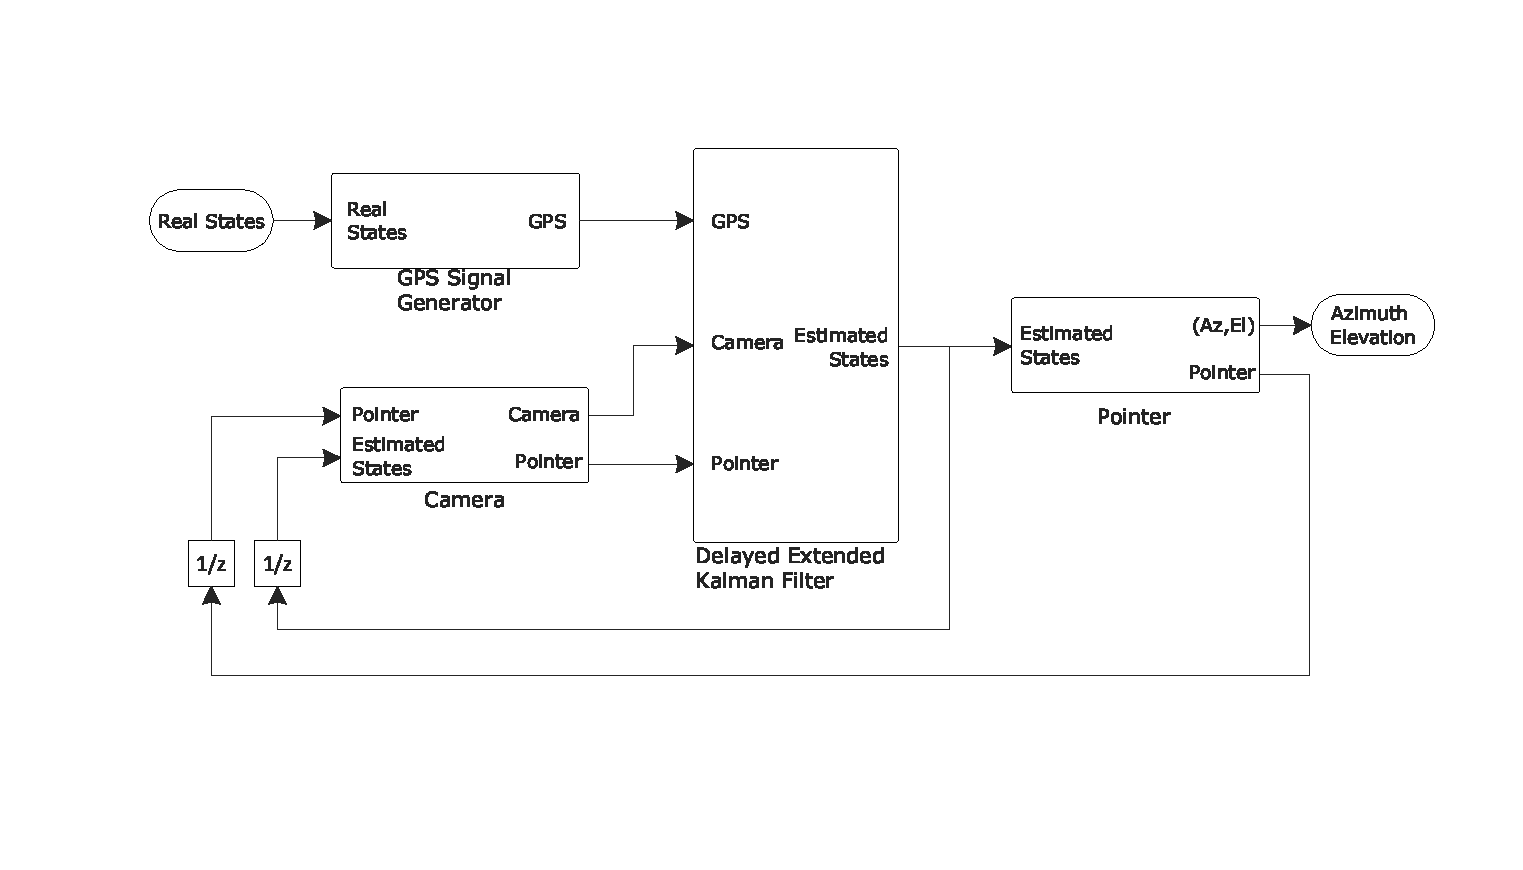
\includegraphics[scale=0.61]{./Simulink/Simulink_AP.eps}
  \label{fig:AP}
  \caption[Antenna Pointer Block]{Antenna Pointer Block. The interaction of each sub-block of the Antenna Pointer Block is shown here. The GPS receives the real measurements, adds noise and delays them. The camera receives the estimated states of the plane and if in the field of view send the position to the DEKF. The filter process all the data and outputs the estimation of the states. Finally the Pointer calculates the azimuth and elevation angles required to point towards the UAV.}
\end{figure}

\subsection{GPS}
This block generates the GPS measurements based in the real states received from the UAV sensor block. First, it reduced the frequency of the data from 100 Hz to 4 Hz, which is the common frequency found in modern GPS. Afterwards, it adds noise to the measurements as described in section \ref{sub:gps_meas_error}. Finally, it waits a random time to send each measurement to the EKF/DEKF block where they are implemented in the estimation.
\pagebreak
\subsection{Camera}
The camera block simulates a camera mounted in the antenna pointer working at a 10 Hz frequency. If the aircraft is in the field of view of the camera, the position in the camera frame is sent to the EKF/DEKF to introduce this data to the estimation of the states. In this simulation we assume that there is an algorithm which detects the UAV as long as it is in the field of view of the camera. The model of this camera is explained in \ref{sub:camera_model}.

\subsection{EKF/DEKF}
This block process the information sent by the GPS and camera blocks to estimate the states of the aircraft. The processing of this data is done by the Delayed Extended Kalman Filter, defined in \ref{sub:DEKF}, which compensates for the delays in the GPS measurements. For comparison purposes the Extended Kalman Filter defined in \ref{sub:EKF} is used, to see how the estimates are impacted if we disregards the delays in the measurements.
In this work, we assume that the delays in the camera measurements can be neglected since the processing unit and the camera are connected directly.  

\subsection{Pointer}
This block calculates the angles to command and the controller of the antenna pointer. First, the pointer uses the estimated states sent by the EKF/DEKF block to calculate the azimuth and elevation angles required to point towards the aircraft. Next, the angles are sent to a simple proportional controller, defined by equations \ref{eq:servo_commands}-\ref{eq:servo_commands}, which actuates the servos in the antenna pointer and feedbacks the actual angles to the camera and the EKF/DEKF blocks. 
\pagebreak
\section{3-D Plot}

The purpose of this block is to recollect all the data and plot the aircraft, the antenna pointer and the field of view of the camera mounted in the antenna pointer in real time.
\begin{figure}[h!]
  \centering
  \includegraphics[scale=0.7]{./Simulink/3Dplot}
  \label{fig:3dplot}
  \caption[Antenna Pointer tracking a UAV.]{Antenna Pointer tracking a UAV. This figure shows a UAV tracking different ground targets using a camera. At the same time, our antenna pointer system, follows the aircraft pointing an antenna and a camera towards it. This graphic was generated using Matlab and Simulink.}
\end{figure}